\chapter{音、量子振動子、そして第二法則}

\lectureoverview{第二法則が目的地であるが、その道を準備する二つの具体的な計算がある。音速は、熱力学的な導関数がどのようにして観測可能な運動になるかを試すものである。次に調和振動子は、剛い自由度に対する古典的な等分配の破綻を明らかにし、量子力学がモードを一つずつ励起する仕組みを示す。最後に、可逆な微視的力学と増大するエントロピーの間の見かけの矛盾に戻り、位相空間の流れ、粗視化、カオス、再帰を用いて、第二法則を例外のない力学的禁止ではなく、圧倒的に確からしい法則として述べる。}

\section{第二法則に関する約束}

中心的な問題は述べるのは容易だが、説明するのは難しい。ニュートンの方程式は可逆である。ある微視的な履歴が許されるなら、時間反転した履歴もまた許される。それにもかかわらず第二法則は、巨視的な過程には好ましい向きがあり、それは通常増大するエントロピーによって特徴づけられると述べている。我々はその緊張に至るであろうが、すぐではない。まず統計力学が具体的な情報を生み出すのを見て、その後、初等的な計算の中で、古典物理学が量子物理学に道を譲らざるを得なかった歴史的な難問に出会う方がよい。

第一の例は数値的で意図的に粗い。希薄気体中の音速を見積もる。第二の例はその仮定の範囲内で厳密である。熱浴中の調和振動子の平均エネルギーを計算する。振動子は等分配から量子化されたエネルギー準位へ、一つのモードから無限に多くのモードへ、そして最後に多粒子系がその初期状態を忘れるとはどういうことかという問いに戻ることになる。

\section{音速の分子的スケール}

希薄気体中の小さな過密度を想像せよ。分子が混み合った領域を離れるためにそれは広がるので、その伝播速度は分子速度と同程度であるはずである。等分配は一分子の運動エネルギーを与える。\begin{equation}
 \frac{3}{2}k_B T
 =\frac{1}{2}m\expect{v^2},
 \qquad
 \expect{v^2}=\frac{3k_B T}{m}.
 \label{eq:sm7-molecular-speed}
\end{equation}
ここで温度は絶対零度から測られ、実験室単位を望むので\(k_B\)が復元されている。この議論はスケールの見積もりにすぎない。分子の二乗平均平方根速度それ自体は集団的な音波の速度ではない。

より系統的な導出では、気体の小さな要素を考える。反対側の面にかかる圧力が等しくないため正味の力が生じ、その加速度は質量密度に反比例する。結果は次の形をとる。\begin{equation}
 c_s^2=
 \left(\frac{\partial P}{\partial \rho_m}\right)_{\cal C},
 \qquad
 \rho_m=m\rho,
 \label{eq:sm7-sound-general}
\end{equation}
ここで\(\rho\)は数密度であり、添字\({\cal C}\)は擾乱によって従われる熱力学的条件を指定する。板書の計算では次を用いる。\begin{equation}
 P=\rho k_B T
 \quad\Longrightarrow\quad
 \frac{1}{m}
 \left(\frac{\partial P}{\partial\rho}\right)_T
 =\frac{k_B T}{m}.
 \label{eq:sm7-sound-isothermal}
\end{equation}
これは等温音速の見積もりである。これは\eqref{eq:sm7-molecular-speed}とは、速度の二乗で\(3\)の因子、あるいは速度で\(\sqrt{3}\)だけ異なる。

\begin{figure}[t]
\centering
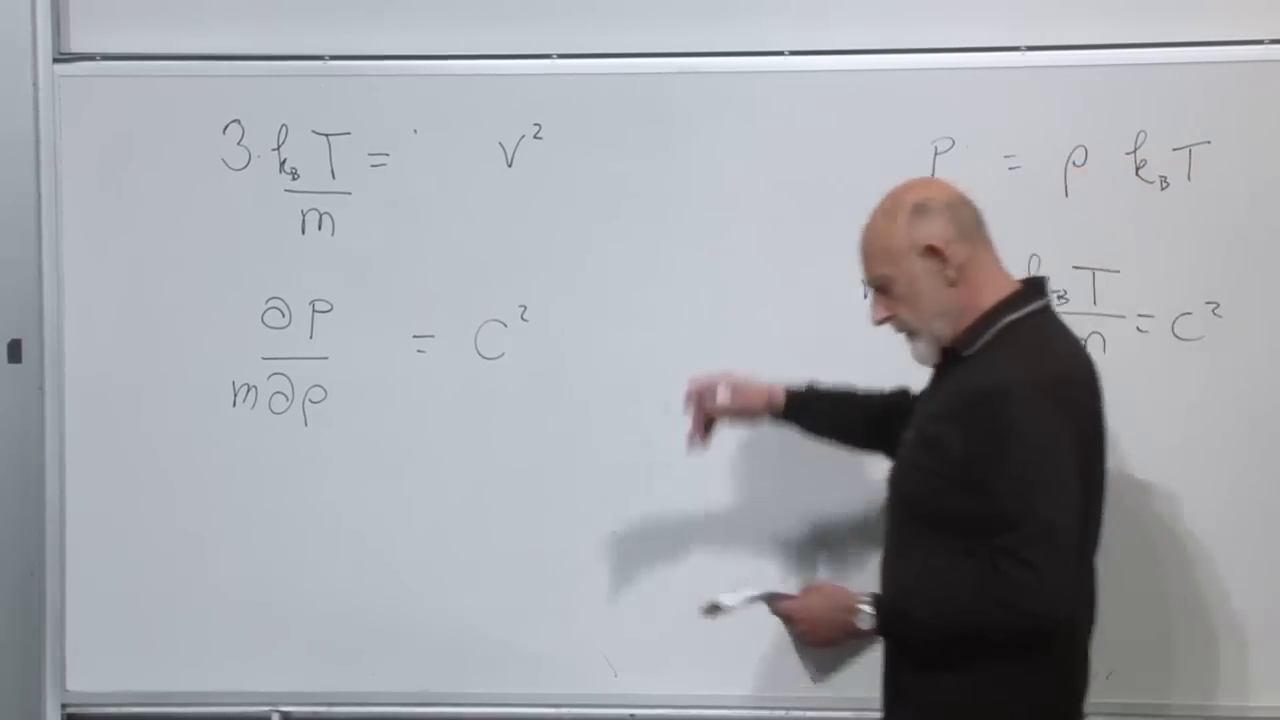
\includegraphics[width=0.90\textwidth]{lecture_07_figure_02.png}
\caption{分子速度の見積もり、圧力の導関数、そして理想気体の代入を一緒に示したもの。}
\lectureframe{00:08:55}
\end{figure}

重要な改良がある。小振幅の音波は通常、隣接する要素間で熱が流れるよりも速く気体を圧縮・膨張させる。したがって局所的な運動は近似的に断熱的であり、等温的ではない。\begin{equation}
 c_s^2=
 \left(\frac{\partial P}{\partial\rho_m}\right)_S.
 \label{eq:sm7-sound-adiabatic}
\end{equation}
断熱指数\(\gamma\)をもつ理想気体では、\begin{equation}
 P\rho_m^{-\gamma}=\text{constant},
 \qquad
 c_s^2=\gamma\frac{P}{\rho_m}
       =\gamma\frac{k_B T}{m}.
 \label{eq:sm7-sound-ideal-adiabatic}
\end{equation}
室温の二原子空気では\(\gamma\simeq 7/5\)である。したがって固定温度の計算は有用な第一の見積もりであり、断熱的な導関数が物理的に適切な改良を与える。

粗い値を用いると\begin{equation}
\begin{aligned}
 k_B&\simeq1.3\times10^{-23}\ {\rm J\,K^{-1}},
 &T&\simeq300\ {\rm K},\\
 m_{\rm air}&\simeq4\times10^{-26}\ {\rm kg}.&&
\end{aligned}
 \label{eq:sm7-air-data}
\end{equation}
分子の見積もりはおよそ\(500\ {\rm m\,s^{-1}}\)である。ここでの温度はケルビン単位の絶対温度でなければならず、華氏のようなオフセット尺度ではない。よく知られた音速は\(300\ {\rm m\,s^{-1}}\)の程度であり、断熱理想気体の式は室温でおよそ\(340\ {\rm m\,s^{-1}}\)を与える。したがって粗い計算は正しい物理的スケールを見出したことになる。

\begin{figure}[t]
\centering
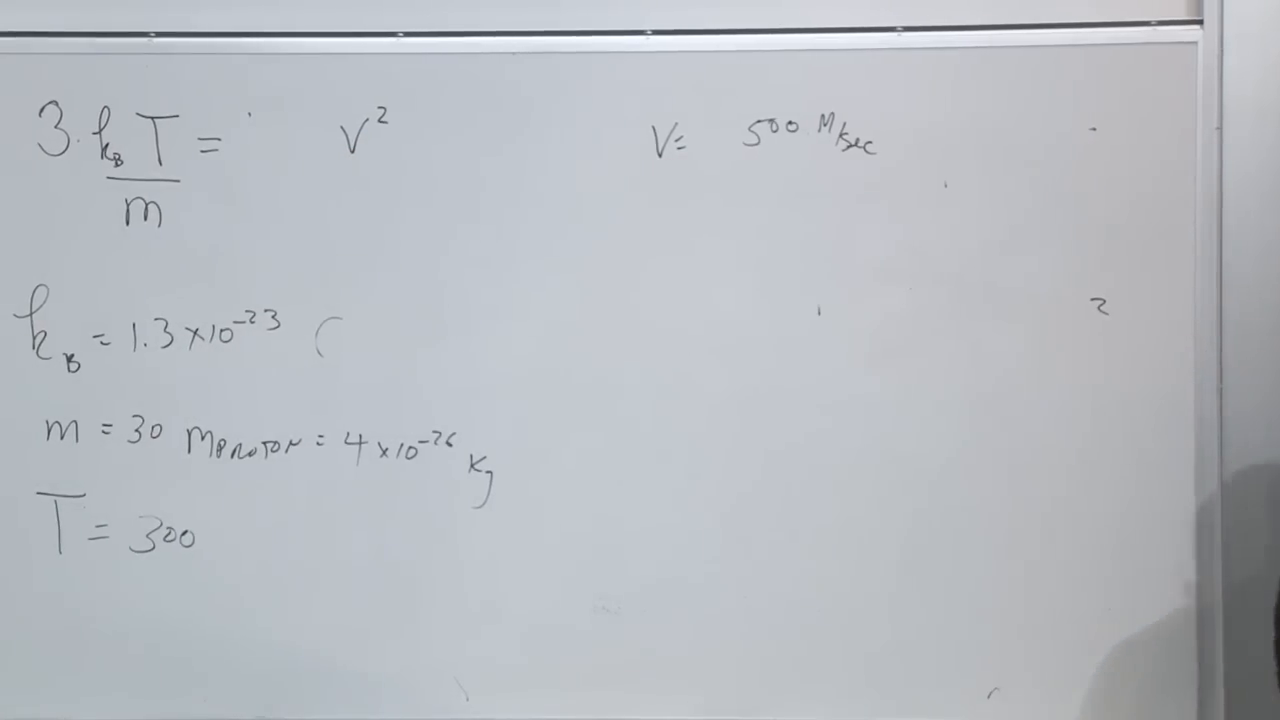
\includegraphics[width=0.90\textwidth]{lecture_07_figure_03.png}
\caption{ボルツマン定数、およそ\(30\)陽子質量に近い有効分子質量、そして\(T\simeq300\ {\rm K}\)を用いた室温空気の見積もり。}
\lectureframe{00:10:55}
\end{figure}

微視的な説明が得られるずっと以前から、密度の関数としての圧力の測定から音速を決定することができた。統計的な議論は、その結果得られる巨視的な速度が個々の分子の熱速度によって定まるという際立った解釈を付け加える。

\begin{classroomqa}
\audiencequestion{中性子は分子質量に加えるべきなのか、また窒素についての数\(14\)は陽子だけを数えているのか。}
\lecturerresponse{引用された原子量はすでに陽子と中性子を数えている。分子状窒素は原子量およそ\(14\)の原子を2個含むので、その質量はおよそ\(28\)陽子質量である。この見積もりには\(28\)を\(30\)に丸めるだけで十分である。
\lecturetimestamp{00:10:58--00:11:16}}
\end{classroomqa}

\begin{classroomqa}
\audiencequestion{因子\(3\)は3つの並進方向から来たが、音は1つの方向に伝播する。それなら\(3\)の因子は除くべきではないか。}
\lecturerresponse{それは、3次元の二乗平均平方根分子速度を1次元の伝播速度と同一視してはならないことを正しく警告している。冒頭の議論は桁程度の描像にすぎなかった。制御された答えは、圧力の導関数と、波に適した熱力学的条件から得られる。
\lecturetimestamp{00:11:12--00:12:00}}
\end{classroomqa}

\begin{classroomqa}
\audiencequestion{その導関数は、波の間、温度が一定に保たれると仮定したのか。}
\lecturerresponse{示された理想気体の代入はそうした。温度を固定することは、ごく小さな擾乱に対するもっともらしい暫定的見積もりである。標準的な精密化は、通常の音が近似的に断熱的であるというものであり、それにより等温導関数が\(\left(\partial P/\partial\rho_m\right)_S\)に置き換わる。
\lecturetimestamp{00:12:59--00:14:01}}
\end{classroomqa}

\begin{classroomqa}
\audiencequestion{圧力と密度の変動がどちらも小さいなら、それらの導関数も小さくなるのか。}
\lecturerresponse{いいえ。導関数は、無限小極限における2つの小さな変動の比である。\(\delta P\)と\(\delta\rho\)はどちらも小さくあり得るが、\(\delta P/\delta\rho\)は有限のままであり、波の速度を定める。
\lecturetimestamp{00:14:03--00:14:23}}
\end{classroomqa}

\begin{classroomqa}
\audiencequestion{気体が圧縮されると、気体から液体や固体へ移る場合のように、音速は上昇すべきなのか。}
\lecturerresponse{はい。導関数は考察中の状態で評価され、\(P(\rho,T)\)は線形のままでいる必要はない。分子が互いに近くに押し込まれると、状態方程式は非理想的になり、\(\partial P/\partial\rho\)はかなり大きくなり得る。
\lecturetimestamp{00:14:25--00:15:13}}
\end{classroomqa}

\begin{classroomqa}
\audiencequestion{値\(500\ {\rm m\,s^{-1}}\)はあらゆる圧力で使えるのか。}
\lecturerresponse{いいえ。それは理想気体方程式が有用な近似となる低密度領域に属する。密度のより高い冪が\(P(\rho,T)\)に入ると、導関数、したがって音速は圧力と密度に依存する。
\lecturetimestamp{00:15:14--00:16:29}}
\end{classroomqa}

\begin{classroomqa}
\audiencequestion{音がほぼ分子速度で広がるという元の描像も、密度が増すにつれて破綻するのか。}
\lecturerresponse{おそらくそうである。その描像は希薄気体に合わせて仕立てられたものである。高密度では集団的相互作用がますます重要になり、まさにそのために状態方程式の導関数がより一般的な記述となるのである。
\lecturetimestamp{00:16:32--00:16:53}}
\end{classroomqa}

\begin{classroomqa}
\audiencequestion{なぜ窒素分子の質量は\(28\)ではなく、およそ\(30\)陽子質量と書かれたのか。}
\lecturerresponse{見積もりに適した数値精度だけが必要なので、\(28\)は\(30\)に丸められた。元の\(500\ {\rm m\,s^{-1}}\)という見積もりを\(\sqrt{3}\simeq1.7\)で割っても\(300\ {\rm m\,s^{-1}}\)に近くなるが、補正を計算する制御された方法は断熱導関数である。
\lecturetimestamp{00:16:54--00:17:27}}
\end{classroomqa}

\section{熱浴中の1つの古典的振動子}

ここで、自由に並進する分子を1つの調和振動子に置き換え、その他すべてを熱浴として扱う。ばねについた質量が直接の描像であるが、この模型ははるかに広い。電磁空洞モードは振動し、結晶中の原子は振動し、平衡からわずかにずらされたほとんど任意の安定な系は、主要な次数で調和運動を行う。

平衡からの変位\(x\)、運動量\(p\)、質量\(m\)、ばね定数\(\kappa\)を用いると、ハミルトニアンは
\begin{equation}
 H(x,p)=\frac{p^2}{2m}+\frac{\kappa x^2}{2},
 \qquad
 \omega=\sqrt{\frac{\kappa}{m}}.
 \label{eq:sm7-classical-hamiltonian}
\end{equation}
である。熱浴は\(T\)を固定し、この時点から再び\(k_B=1\)を用いるので、\(\beta=1/T\)となる。室温と平衡にある振動子は\(300\ {\rm K}\)付近の温度をもち、液体ヘリウムに浸されたものはわずか数ケルビンの温度しかもたない。太陽の中心に置かれたと仮定したばねはばねとして生き残らないであろうが、この例は環境の役割を明瞭にする。ボルツマン重みは因子分解する:
\begin{equation}
 e^{-\beta H}
 =e^{-\beta p^2/(2m)}
  e^{-\beta\kappa x^2/2}.
 \label{eq:sm7-factorized-weight}
\end{equation}

\begin{figure}[t]
\centering
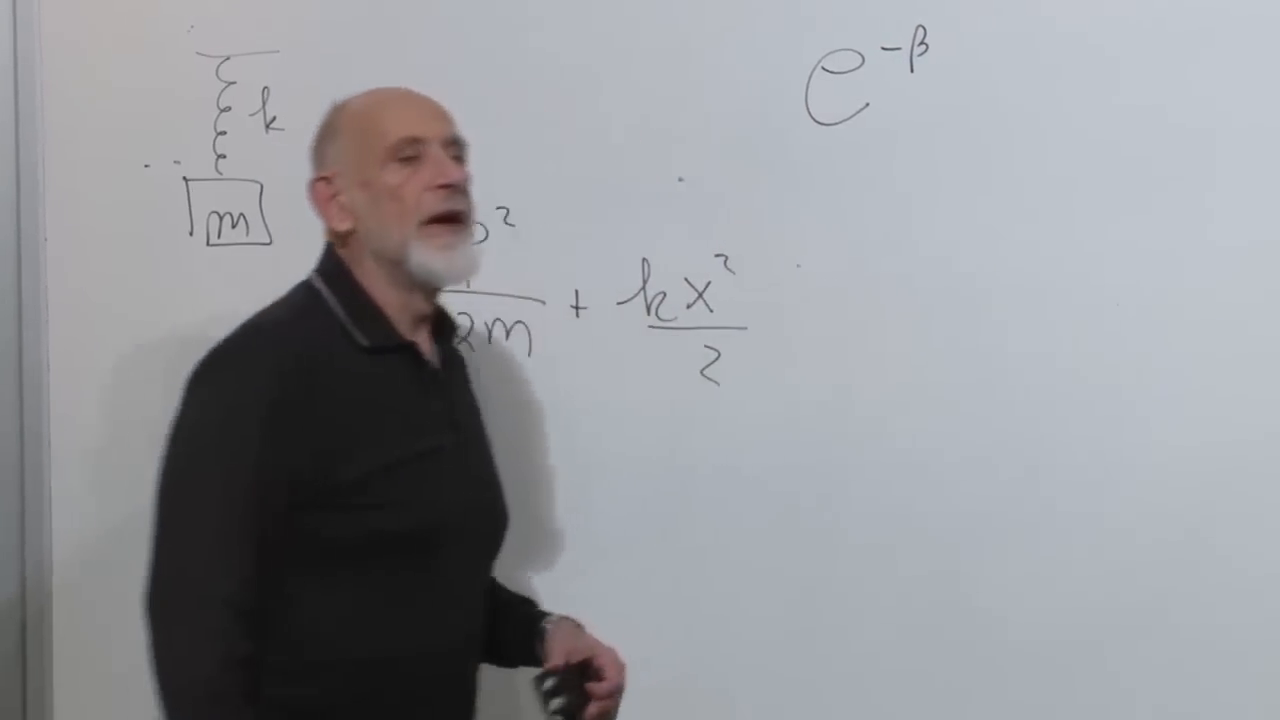
\includegraphics[width=0.90\textwidth]{lecture_07_figure_04.png}
\caption{ばね-質量振動子とその運動エネルギーおよびポテンシャルエネルギーのハミルトニアン。}
\lectureframe{00:20:55}
\end{figure}

自由気体とは異なり、位置積分は単に容器の体積を与えるだけではない。復元ポテンシャルが各変位に重みを付ける：
\begin{equation}
 Z_{\rm cl}
 =\frac{1}{h}\int_{-\infty}^{\infty}dp
             \int_{-\infty}^{\infty}dx\,
 e^{-\beta p^2/(2m)}
 e^{-\beta\kappa x^2/2}.
 \label{eq:sm7-classical-z}
\end{equation}
因子\(1/h\)は一次元古典分配関数を無次元にする。これは\(\beta\)に依存せず平均エネルギーに影響し得ないため、板書の計算では省略されている。

\begin{figure}[t]
\centering
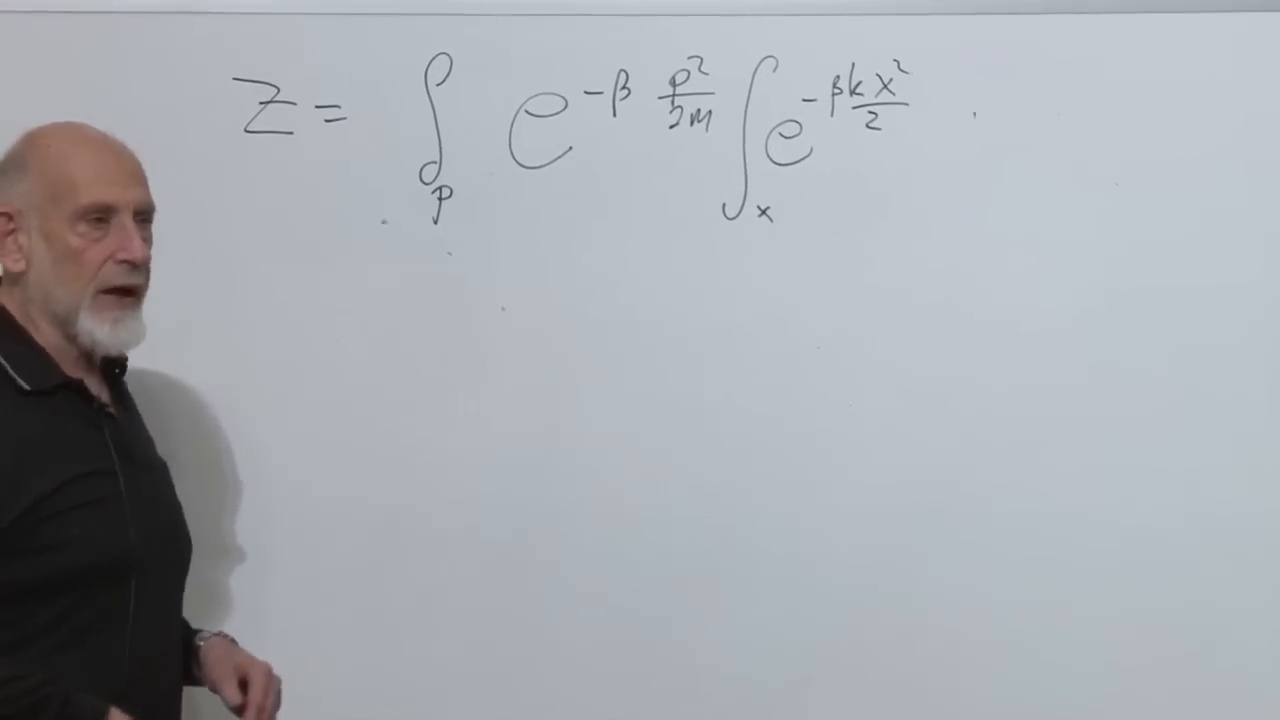
\includegraphics[width=0.90\textwidth]{lecture_07_figure_05.png}
\caption{運動量と変位のガウス積分に分離された古典振動子の分配関数。}
\lectureframe{00:22:55}
\end{figure}

運動量積分に対しては
\begin{equation}
 q=\sqrt{\frac{\beta}{2m}}\,p,
 \qquad
 dp=\sqrt{\frac{2m}{\beta}}\,dq.
 \label{eq:sm7-p-gaussian-substitution}
\end{equation}
と置く。位置積分に対しては
\begin{equation}
 y=\sqrt{\frac{\beta\kappa}{2}}\,x,
 \qquad
 dx=\sqrt{\frac{2}{\beta\kappa}}\,dy.
 \label{eq:sm7-x-gaussian-substitution}
\end{equation}
と置く。\(\int_{-\infty}^{\infty}e^{-u^2}\,du=\sqrt{\pi}\)であるから、板書で用いられる規格化されていない位相空間積分は
\begin{equation}
 \int dp\,dx\,e^{-\beta H}
 =\frac{2\pi}{\beta}\sqrt{\frac{m}{\kappa}}
 =\frac{2\pi}{\beta\omega}.
 \label{eq:sm7-classical-z-unnormalized}
\end{equation}
となる。位相空間のセルを復元すると、
\begin{equation}
 Z_{\rm cl}=\frac{2\pi}{h\beta\omega}
           =\frac{1}{\beta\hbar\omega}.
 \label{eq:sm7-classical-z-normalized}
\end{equation}

エネルギーに対しては\(\beta\)依存性のみが重要である：
\begin{equation}
 \begin{aligned}
 \log Z_{\rm cl}&=\text{constant}-\log\beta,\\
 \expect{H}
 &=-\frac{\partial\log Z_{\rm cl}}{\partial\beta}\\
 &=\frac{1}{\beta}=T.
 \end{aligned}
 \label{eq:sm7-classical-energy}
\end{equation}

\begin{figure}[t]
\centering
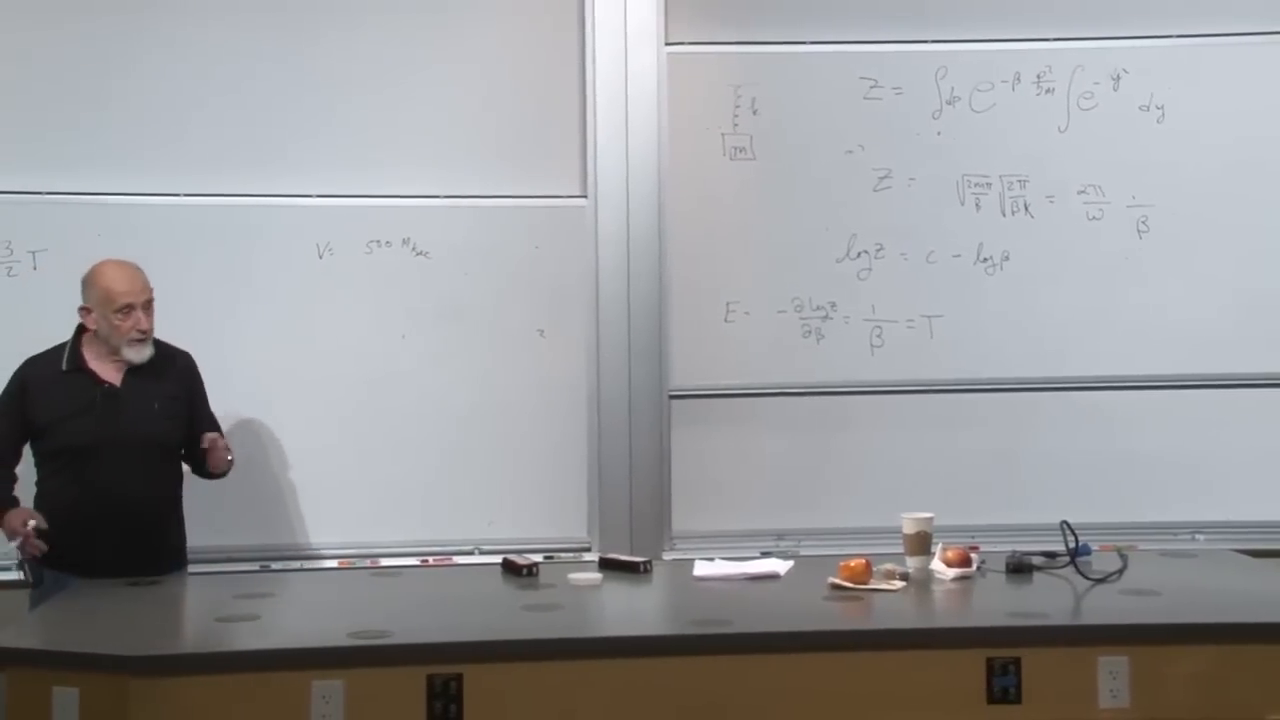
\includegraphics[width=0.90\textwidth]{lecture_07_figure_06.png}
\caption{右の板書における完全な古典的連鎖：ガウス分解、\(Z\propto(\beta\omega)^{-1}\)、そして\(\expect{H}=1/\beta=T\)。}
\lectureframe{00:30:15}
\end{figure}

これは一つの空間的振動子であるから、\(3\)の因子は存在しない。また二つの独立な二次項があるため、\(1/2\)の残りの因子も存在しない。各ガウス積分は\(T/2\)に寄与する：
\begin{equation}
 \expect{K}=\frac{T}{2},
 \qquad
 \expect{U}=\frac{T}{2},
 \qquad
 \expect{H}=T.
 \label{eq:sm7-equipartition-oscillator}
\end{equation}
これが最も有用な形でのエネルギー等分配則である：古典ハミルトニアンにおける各独立な二次項は\(T/2\)に寄与する。

答えは\(m\)と\(\kappa\)の両方に依存しない。運動自体はこれらのパラメータに依存する：
\begin{equation}
 \expect{p^2}=mT,
 \qquad
 \expect{x^2}=\frac{T}{\kappa},
 \qquad
 \expect{\dot{x}^2}=\frac{T}{m}.
 \label{eq:sm7-classical-fluctuations}
\end{equation}
したがって、より重い質量はよりゆっくりと運動し、より硬いばねはより小さな振幅を持つが、平均エネルギーは依然として\(T\)である。\(\kappa\)が途方もなく大きくなると、このことは厄介になる。動かないほど硬いばねは凍結した拘束のように見えるべきであるのに、古典的なエネルギー等分配は依然としてそれにエネルギー\(T\)を割り当てる。

\begin{classroomqa}
\audiencequestion{\(\kappa\to\infty\)のとき、分配関数はゼロに近づく。それでもその対数はどのようにして用いることができるのか？}
\lecturerresponse{\(\kappa\)を有限だが任意に大きく保つ。\(\log Z\)への寄与は加法的であり\(\beta\)に依存しないため、\(\beta\)による微分は依然として\(T\)を与える。極限における不快感は現実のものである：古典的計算は内部的に整合しているが、非常に硬い振動子に必要な自然の特徴を欠いている。
\lecturetimestamp{00:34:01--00:34:54}}
\end{classroomqa}

\begin{classroomqa}
\audiencequestion{理想気体の分配関数には\(N!\)が必要であった。ここにも同様の階乗があるべきだろうか？}
\lecturerresponse{いいえ。我々は一つの指定された振動子を研究しているのであり、\(N\)個の同一粒子を並べ替えているのではない。多くの独立なラベル付きモードに対しては、分配関数は掛け合わされる。不可弁別因子は別の数え上げ問題に属する。
\lecturetimestamp{00:35:03--00:35:40}}
\end{classroomqa}

\section{なぜ古典的エネルギー等分配は危機であったか}

実在の分子は構造のない点ではない。二原子分子は振動し得る結合を含み、したがって内部振動子を持つ。素朴な古典的勘定では、通常の温度においてさえそのモードに追加の熱エネルギーを割り当てることになる。意図的に図式的な勘定では、一つの振動子を活性化すると\(3T/2\)のエネルギーが\(5T/2\)に向かって上昇する。精密な熱容量の記帳は回転自由度も含み、エネルギーとその温度微分を区別しなければならない。決定的な実験的事実はより単純である：硬い内部モードは、古典的エネルギー等分配が要求するようには低温で寄与しなかった。

分子が内部構造を持つことを否定するか、それは不合理であるが、あるいは古典力学に何かが欠けていることを認めるかである。欠けているものは量子力学である。我々が必要とするのはそのほんのわずかである：調和振動子が等間隔のエネルギー準位を持つということだけである。

\section{量子振動子}

まずエネルギーの原点をずらし、励起スペクトルを
\begin{equation}
 E_n^{\rm exc}=n\hbar\omega,
 \qquad n=0,1,2,\ldots.
 \label{eq:sm7-shifted-spectrum}
\end{equation}
と書く。分配関数は今や位相空間積分ではなく真の和である：
\begin{align}
 Z_{\rm exc}
 &=\sum_{n=0}^{\infty}e^{-\beta n\hbar\omega} \notag\\
 &=1+x+x^2+\cdots
  =\frac{1}{1-x},
 \qquad x=e^{-\beta\hbar\omega}, \notag\\
 &=\frac{1}{1-e^{-\beta\hbar\omega}}.
 \label{eq:sm7-quantum-z}
\end{align}

\begin{figure}[t]
\centering
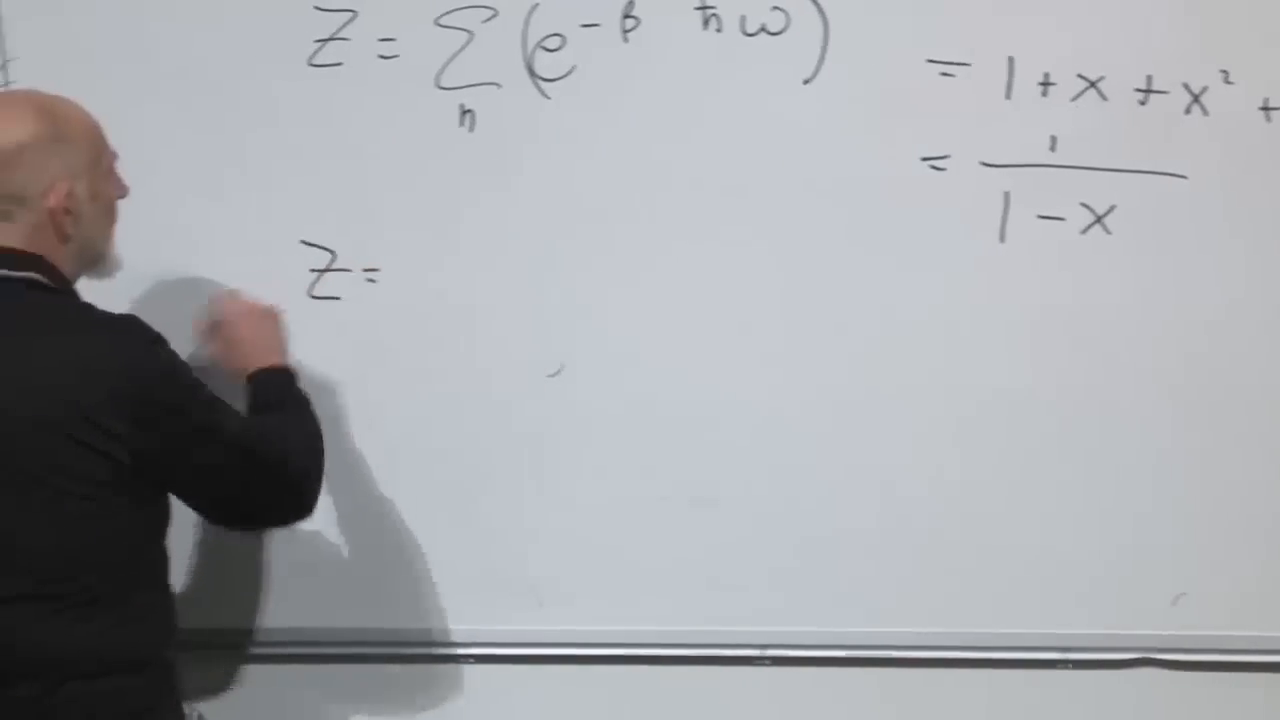
\includegraphics[width=0.90\textwidth]{lecture_07_figure_07.png}
\caption{等間隔準位と量子振動子分配関数の幾何級数による評価。}
\lectureframe{00:42:05}
\end{figure}

微分すると平均励起エネルギーが得られる：
\begin{align}
 E_{\rm exc}
 &=-\frac{\partial\log Z_{\rm exc}}{\partial\beta}
  =-\frac{1}{Z_{\rm exc}}
    \frac{\partial Z_{\rm exc}}{\partial\beta}
 \notag\\
 &=\hbar\omega\,
   \frac{e^{-\beta\hbar\omega}}
        {1-e^{-\beta\hbar\omega}}
  =\frac{\hbar\omega}{e^{\beta\hbar\omega}-1}.
 \label{eq:sm7-quantum-energy}
\end{align}

\begin{figure}[t]
\centering
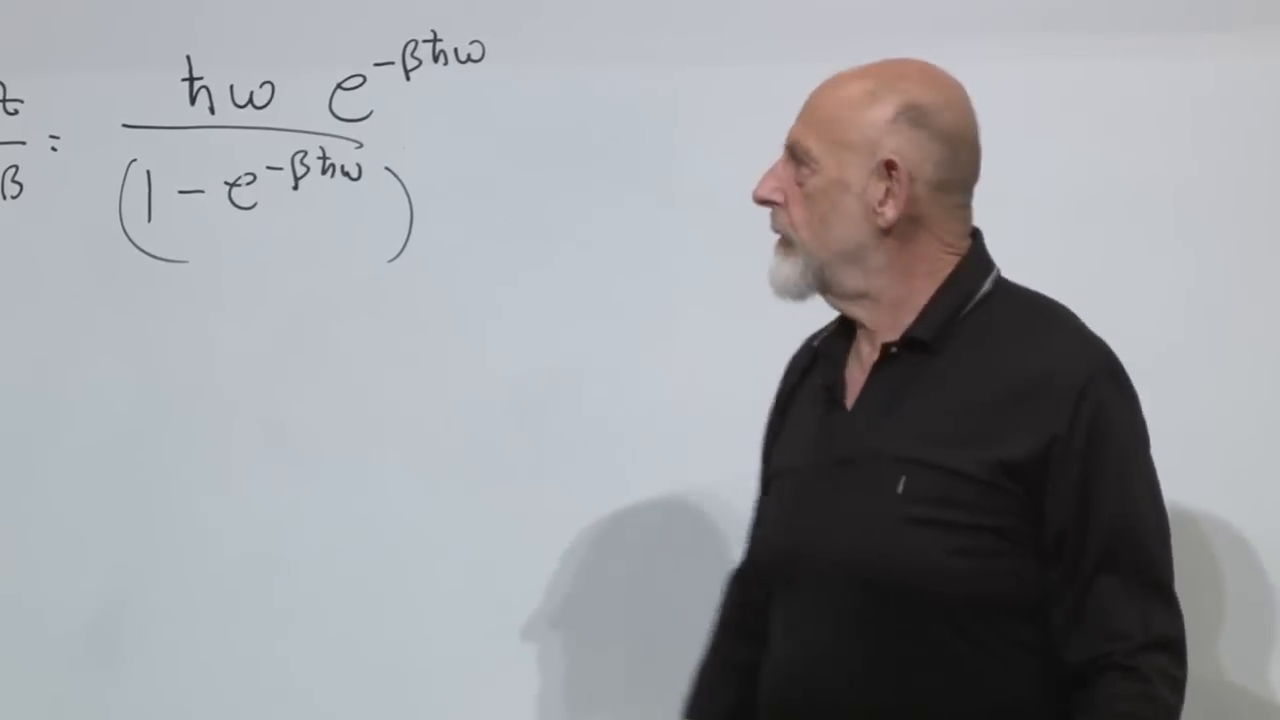
\includegraphics[width=0.90\textwidth]{lecture_07_figure_08.png}
\caption{量子分配関数の\(\beta\)微分から得られる熱励起エネルギー。}
\lectureframe{00:46:05}
\end{figure}

\subsection{高温}

\(\beta\hbar\omega\ll1\)のとき、
\begin{equation}
 e^{-\beta\hbar\omega}
 =1-\beta\hbar\omega
  +O\!\left((\beta\hbar\omega)^2\right).
 \label{eq:sm7-high-t-expansion}
\end{equation}
\eqref{eq:sm7-quantum-energy}の分子は\(\hbar\omega\)に近づき、分母は主要項で\(\beta\hbar\omega\)である。したがって
\begin{equation}
 E_{\rm exc}\simeq\frac{1}{\beta}=T.
 \label{eq:sm7-high-t-energy}
\end{equation}
量子論的答えは、多くの準位間隔が熱エネルギーの中に収まるとき、古典的エネルギー等分配を回復する。

\subsection{低温}

\(\beta\hbar\omega\gg1\) のとき、指数関数は極めて小さい：
\begin{equation}
 E_{\rm exc}
 \simeq\hbar\omega e^{-\beta\hbar\omega}.
 \label{eq:sm7-low-t-energy}
\end{equation}
振動子の熱励起は指数関数的に抑制される。ずらした表記ではほとんどゼロである；物理的な零点エネルギーは以下で復元される。

\begin{figure}[t]
\centering
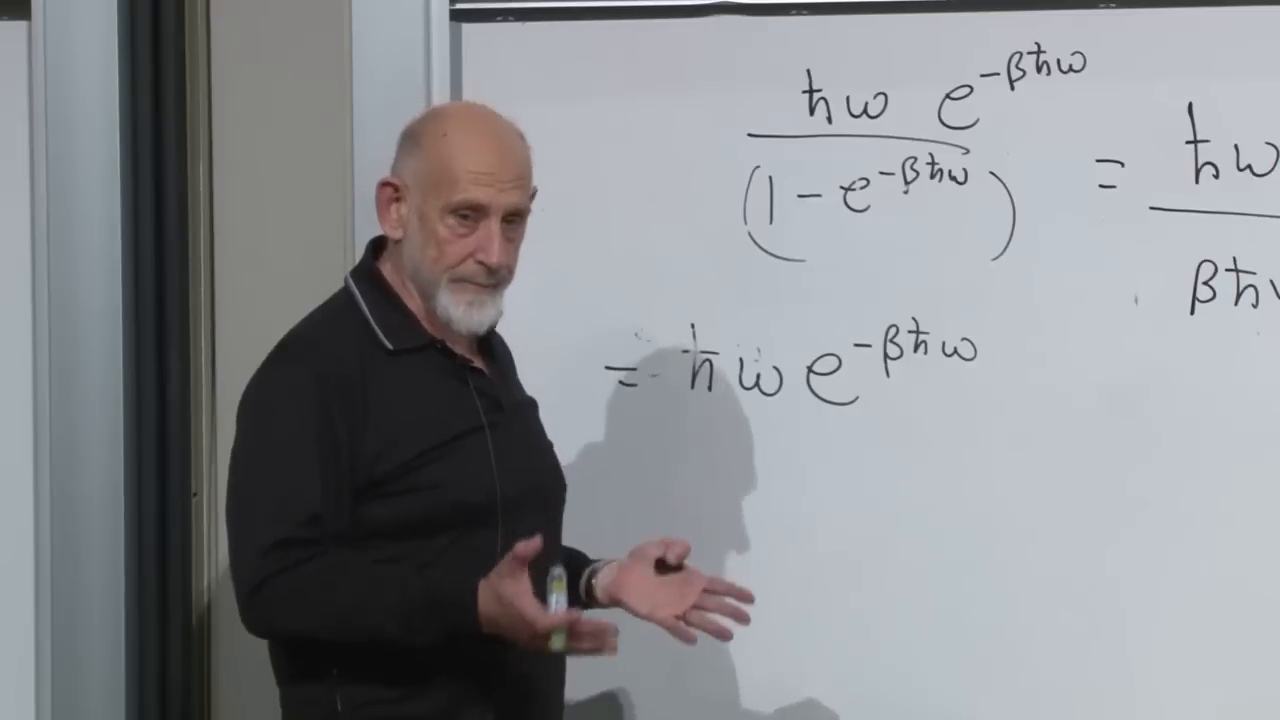
\includegraphics[width=0.90\textwidth]{lecture_07_figure_09.png}
\caption{低温展開：最初の熱励起は \(e^{-\beta\hbar\omega}\) によって抑制される。}
\lectureframe{00:51:55}
\end{figure}

クロスオーバーは次が成り立つときに起こる：
\begin{equation}
 \beta\hbar\omega\sim1,
 \qquad\text{or equivalently}\qquad
 T\sim\hbar\omega.
 \label{eq:sm7-crossover}
\end{equation}
この条件には直接的な意味がある。古典的な等分配則では振動子のエネルギーは \(T\) となる。そのスケールが1つの準位間隔を下回ると、量子効果は避けられなくなる。したがって
\begin{equation}
\begin{aligned}
 \hbar\omega\gg T&:\quad \text{frozen and quantum},\\
 \hbar\omega\ll T&:\quad \text{active and classical}.
\end{aligned}
 \label{eq:sm7-regimes}
\end{equation}
より硬いばねはより大きな \(\omega=\sqrt{\kappa/m}\) をもつので、古典的に振る舞うにはより高い温度を必要とする。

\section{物質を加熱すると自由度が現れる}

低温では、二原子分子はその硬い結合振動が凍結しているため、熱的に点粒子のように振る舞うことができる。\(T\) が \(\hbar\omega\) を超えて上昇すると、振動モードが活性化する。回転モードはより低いスケールで活性化するかもしれない；さらに高い温度ではより多くの内部運動が現れ、最終的には原子が電離する。加熱は単に固定されたモードのリストにより多くのエネルギーを注ぎ込むだけではない。それは低温では見えなかった自由度を明らかにする。

想像上の入れ子分子がこの点を鮮明にする。2つの原子は硬いばねで結ばれているが、見かけ上の1つの原子はそれ自体、さらに硬いばねで結ばれた対である。低い \(T\) では、両方の構造は点的に見える。最初のしきい値で外側の振動が現れる；2番目のしきい値で内側の構造が現れる。系の複雑さは、一度に1つのエネルギー・スケールずつ明らかになる。

\begin{classroomqa}
\audiencequestion{振動子がすでに古典的領域にあるとき、さらに加熱するとばねが硬くなったり振動数が変化したりするのか？}
\lecturerresponse{いいえ。ばね定数と振動数は固定されたままである。より高い温度はより大きな典型的運動量と振幅を生み、したがってより大きなエネルギーを生む。硬さは古典的法則が始まる温度を決めるのであって、温度に依存してばねが硬くなるのではない。
\lecturetimestamp{01:03:17--01:05:11}}
\end{classroomqa}

\subsection{結晶とアインシュタインの比熱}

結晶は非常に多くの振動モードを含む。古典的な等分配則はすべての活性な振動子に \(T\) スケールのエネルギーを割り当てるため、低温での熱容量を過大評価する。アインシュタインの 1907 模型は結晶振動を量子力学的に扱い、熱エネルギーがそれらの準位間隔に達するまでなぜ抑制されるかを示した。より正確な固体模型はモード振動数の分布を許すが、凍結の原理はすでにアインシュタインの計算に存在している。

\begin{classroomqa}
\audiencequestion{これはアインシュタインがノーベル賞を受賞した仕事であり、量子力学が確立された後に初めて現れたのか？}
\lecturerresponse{いいえ。ノーベル賞の授賞理由は光電効果に関するものであった。比熱模型は 1907 に発表され、量子力学の完全な基礎が理解されるずっと前であった。アインシュタインは、後に成熟した理論の側面に反対したにもかかわらず、決定的な量子のアイデアを受け入れ、発展させた。
\lecturetimestamp{00:58:38--01:03:16}}
\end{classroomqa}

\begin{classroomqa}
\audiencequestion{古典統計力学は、離散状態の和を位置と運動量にわたる一見一様な積分に置き換えた。何がその状態の数え方を正当化するのか？}
\lecturerresponse{究極的な正当化は量子力学から来る。高温極限では、
\[
 Z_{\rm exc}\simeq\frac{1}{\beta\hbar\omega},
\]
これは無次元の古典的結果
\eqref{eq:sm7-classical-z-normalized} と正確に一致する。準位間隔が分解されないとき、位相空間の量子セルは古典的位相空間測度になる。
\lecturetimestamp{00:59:38--01:03:06}}
\end{classroomqa}

\subsection{弦は無限に多くの振動子を含む}

バイオリンやギターの弦は基準モードに分解される：基本振動、より高い倍音、そして次第に短くなる波長である。数学的には無限に多くの振動子モードが存在する。もし古典的な等分配則がそのすべてにエネルギー \(T\) を割り当てるなら、熱平衡にある弦は無限のエネルギーをもつことになる。量子力学がその破局を防ぐ。最短波長のモードは最も高い振動数をもち、任意の有限温度で凍結したままである；\(T\) が上昇するにつれて次第により多くのモードが活性化する。同じ論理は後に黒体放射の基礎となる。

\begin{figure}[t]
\centering
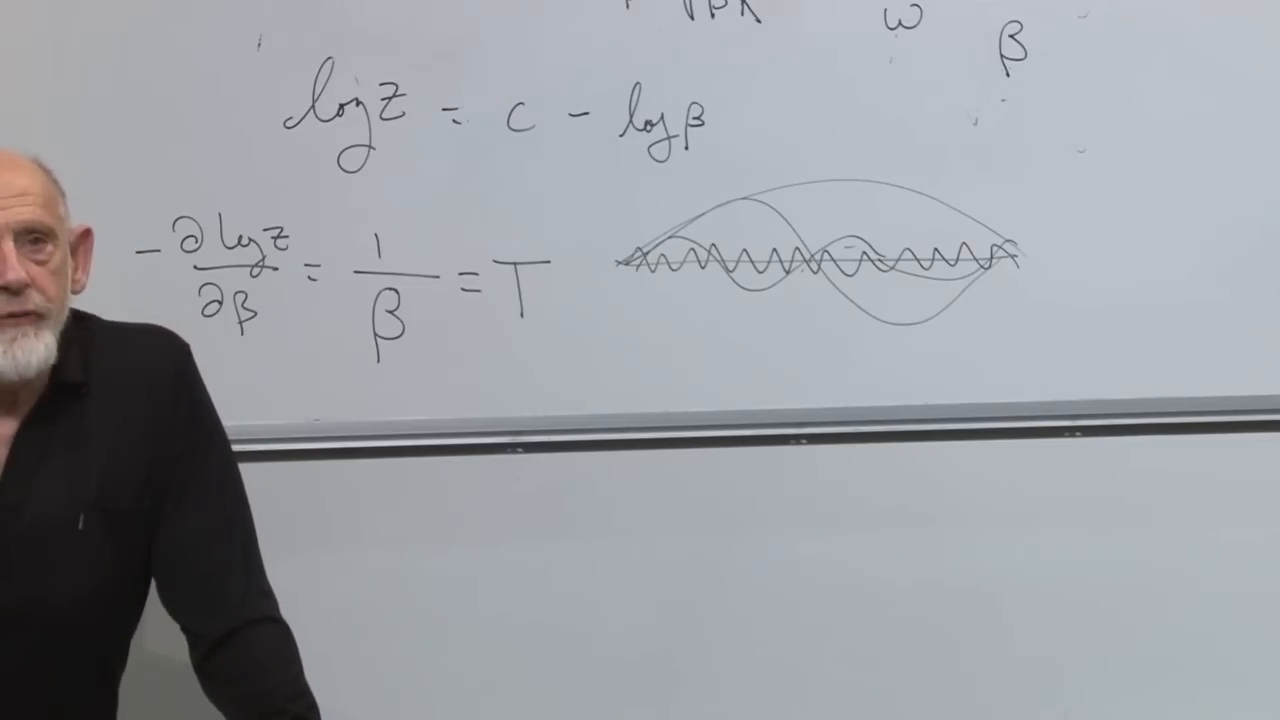
\includegraphics[width=0.90\textwidth]{lecture_07_figure_10.png}
\caption{弦上に重ね合わされたいくつかの基準モード。連続的な弦がなぜ無限の調和振動子の集まりであるかを示している。}
\lectureframe{01:09:30}
\end{figure}

\begin{classroomqa}
\audiencequestion{量子から古典へのクロスオーバーは直接観測できるのか、また加熱によって低温での振る舞いを逆転させることができるのか。}
\lecturerresponse{はい。結晶の比熱の温度依存性によって、振動モードの凍結とそれに続く活性化は明瞭に測定可能となる。
\lecturetimestamp{01:09:11--01:10:13}}
\end{classroomqa}

\begin{classroomqa}
\audiencequestion{多数の振動子に対して、単一振動子の分配関数を各モードごとに繰り返すのか。}
\lecturerresponse{独立なモードに対しては、
\[
\begin{aligned}
 Z_{\rm tot}&=\prod_j Z_j,&
 \log Z_{\rm tot}&=\sum_j\log Z_j,\\
 E_{\rm tot}&=\sum_j E_j.&&
\end{aligned}
\]
\(\hbar\omega_j\gg T\) となるモードは熱的寄与が指数関数的に小さく、しきい値より下のモードは無視できない寄与をする。
\lecturetimestamp{01:10:14--01:11:00}}
\end{classroomqa}

\begin{classroomqa}
\audiencequestion{振動子の零点エネルギー \(\hbar\omega/2\) はどうなったのか。}
\lecturerresponse{物理的な準位は
\[
 E_n=\left(n+\frac12\right)\hbar\omega.
\]
したがって
\[
 \begin{aligned}
 Z_{\rm phys}
 &=e^{-\beta\hbar\omega/2}Z_{\rm exc},\\
 E_{\rm phys}
 &=\frac{\hbar\omega}{2}
  +\frac{\hbar\omega}{e^{\beta\hbar\omega}-1}.
 \end{aligned}
\]
共通のずれは準位の確率、エントロピー、熱容量、熱励起エネルギーを変えないが、絶対平均エネルギーを \(\hbar\omega/2\) だけずらす。\(Z\) における乗因子は \(\beta\) に依存するので、絶対エネルギーを求める場合には捨ててはならない。
\lecturetimestamp{01:11:08--01:11:37}}
\end{classroomqa}

\section{可逆性のパズルとしての第二法則}

ここで、約束した問題に戻ることができる。第二法則は、通常のマクロな発展が不可逆であり、エントロピーが増大する傾向があると述べている。ミクロなハミルトニアン的発展は可逆である。可逆な厳密状態の写像が、どのようにしてマクロ状態の不可逆な法則を生み出すのだろうか。

系を高次元位相空間の一点で表す。
\[
 \Gamma=(q_1,\ldots,q_N,p_1,\ldots,p_N).
\]
我々の知識は通常、厳密な一点ではない。それが体積 \(\Omega_A\) のコンパクトなパッチ \(A\) 上の一様な確率密度であると仮定する。
\begin{equation}
 f(\Gamma)=
 \begin{cases}
  1/\Omega_A,&\Gamma\in A,\\
  0,&\Gamma\notin A.
 \end{cases}
 \label{eq:sm7-uniform-blob}
\end{equation}
\(k_B=1\) とする単位系では、その細粒ギブズエントロピーは
\begin{equation}
 S_{\rm fine}
 =-\int d\Gamma\,f\log f
 =\log\Omega_A.
 \label{eq:sm7-blob-entropy}
\end{equation}
パッチが小さいほど情報が多く、エントロピーは低い。これにより符号が定まる。不確かさが増大すると占有領域が広がり、\(\log\Omega_A\) が増大する。

\begin{figure}[t]
\centering
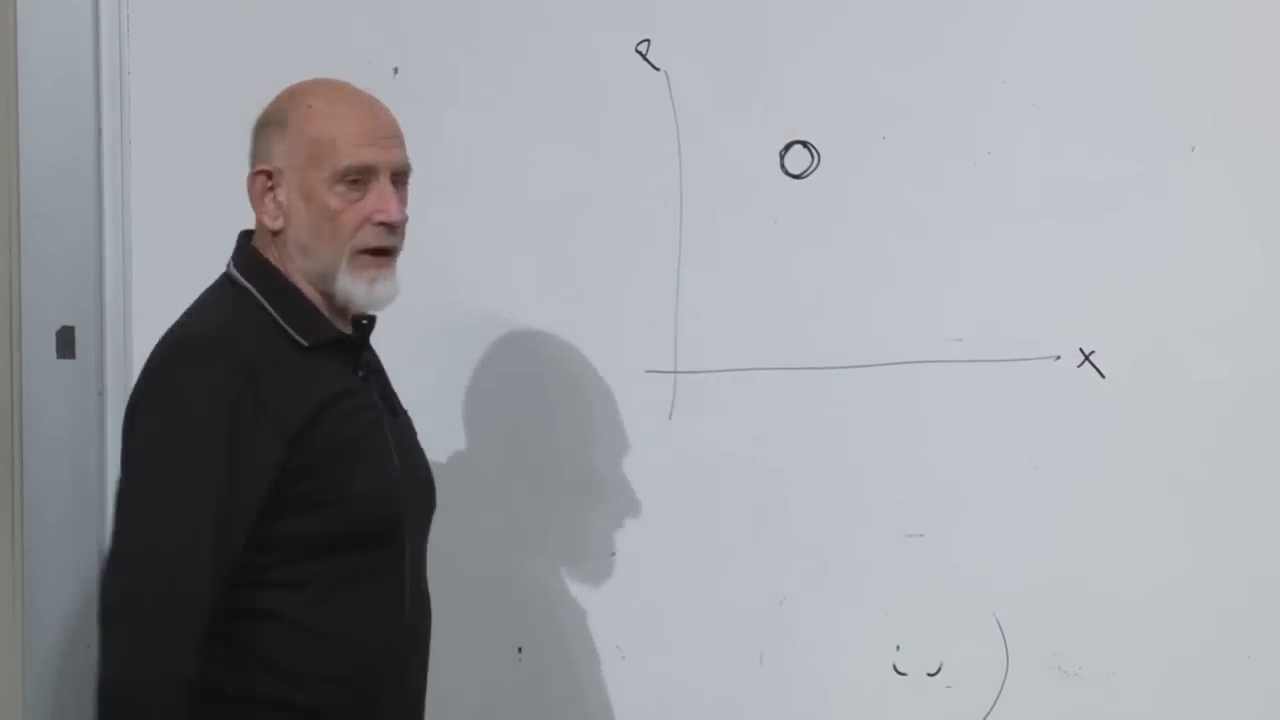
\includegraphics[width=0.90\textwidth]{lecture_07_figure_11.png}
\caption{完全な位置-運動量位相空間の模式的な二次元断面におけるコンパクトな確率パッチ。}
\lectureframe{01:20:20}
\end{figure}

\begin{classroomqa}
\audiencequestion{系は物理的に描かれたパッチの内部にとどまるよう拘束されているのか、またすでに平衡にあるのか。}
\lecturerresponse{いいえ。パッチは初期状態について知られていることを記述するものであり、位相空間における壁ではない。それは平衡分布である必要はない。部屋の隅のタンクに初め閉じ込められた気体は、特殊な非平衡情報の具体的な例である。
\lecturetimestamp{01:14:55--01:15:24}}
\end{classroomqa}

\section{リウヴィル流と粗視化された増大}

リウヴィルの定理は、ハミルトニアン流が位相空間体積を保存すると述べている。厳密なパッチは並進し、伸び、折り畳まれ、極めて薄くなりうるが、
\begin{equation}
 \Omega_{A(t)}=\Omega_{A(0)},
 \qquad
 S_{\rm fine}(t)=S_{\rm fine}(0).
 \label{eq:sm7-liouville}
\end{equation}
離散的な類似物は状態の可逆な置換である。サイコロが二つの状態のいずれかにあると初めに知っている場合、一対一の発展はそれらがどの二つの状態であるかを変えうるが、可能性の数を変えることはない。

現実の記述は有限の分解能をもつ。量子力学は自然な位相空間セルを与えるが、古典的な実験は量子論を持ち出さなくても有限の測定能力をもつ。ハミルトニアン流の下で、パッチは長く薄い蛇になりうる。隣接する折り目の間隔が分解能の尺度を下回ると、我々は分解できない各近傍を粗いセルで置き換える。厳密な占有体積は固定されたままであるが、粗いセルの合併は増大する。
\begin{equation}
 \Omega_{\rm coarse}(t)\geq\Omega_{A(t)},
 \qquad
 S_{\rm coarse}(t)=\log\Omega_{\rm coarse}(t).
 \label{eq:sm7-coarse-entropy}
\end{equation}

\begin{figure}[t]
\centering
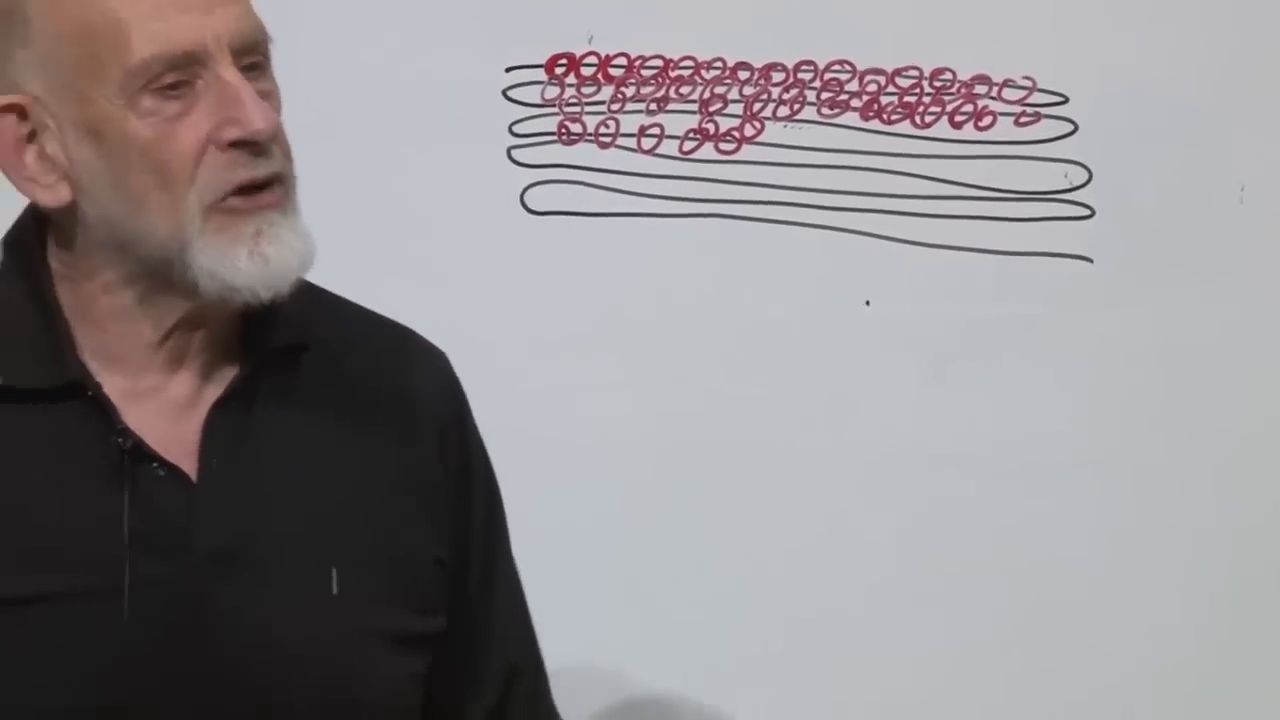
\includegraphics[width=0.90\textwidth]{lecture_07_figure_12.png}
\caption{有限分解能のセルを通して見た体積保存フィラメント。厳密な黒いフィラメントはその面積を保つが、赤い粗いセルはより大きな有効領域を占める。}
\lectureframe{01:22:10}
\end{figure}

\begin{classroomqa}
\audiencequestion{粗いセルが重なり合っている。これはリウヴィルの定理に反するのか。}
\lecturerresponse{いいえ。リウヴィルは厳密なフィラメントを支配し、それは一対一かつ体積保存のままである。重なりは我々のぼやけた記述に属する。我々は状態がどの細い糸に含まれるかという情報を捨て去ったのである。
\lecturetimestamp{01:21:32--01:21:50}}
\end{classroomqa}

有用な類推は綿である。すべての繊維の材料体積はほぼ固定されたままでありうるが、ほぐされた綿の塊は、個々の繊維を分解できない観察者にとって大きな見かけの体積を占める。同様に、位相空間のパッチはより細い触手を成長させ、それらの触手はさらに細い触手を発達させる。任意の固定された有限分解能は、最終的にそれらを追跡できなくなる。

\begin{classroomqa}
\audiencequestion{エントロピーは古典的には増大して見えるだけで、量子力学が基本的な分解能の限界を課すことによってその増大を実在のものにするのだろうか。}
\lecturerresponse{粗視化の議論は量子限界を必要としない。エントロピーは系と、その記述において保持される巨視的な区別とを合わせて指し示す。無限の微視的情報があれば、細視化エントロピーは一定である。いかなる固定された有限の分解能のもとでも、カオス的なフィラメントはやがて分解されなくなり、粗視化エントロピーは増大する。
\lecturetimestamp{01:24:04--01:25:20}}
\end{classroomqa}

\section{カオス、有限の到達可能領域、そして平衡化}

箱の中の気体では、位置は有界である。有限の全エネルギーを固定すれば、たとえすべてのエネルギーが一時的に一つの粒子に集中しても、運動量もまた有界である。したがって、通常の閉じ込めの仮定のもとで、力学的に到達可能なエネルギー殻は有限の測度をもつ。

\begin{figure}[t]
\centering
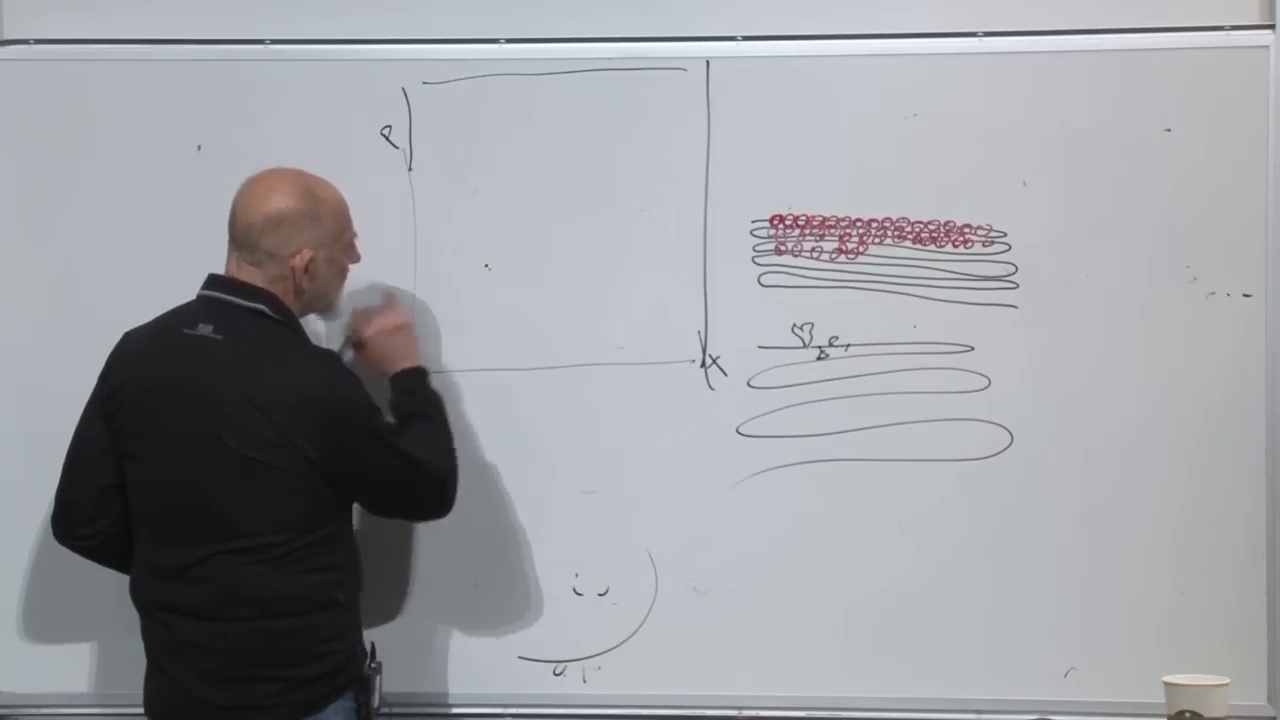
\includegraphics[width=0.90\textwidth]{lecture_07_figure_13.png}
\caption{フィラメントとその粗視化された表現に隣接する、有界な到達可能相空間領域。}
\lectureframe{01:28:10}
\end{figure}

カオス系における近接した初期点は、しばらくは似た履歴をたどるが、その後分離する。ビリヤードのブレイクでは、手球の方向の知覚できないほどの変化がその後の衝突へと写し取られ、差異は複合して最終的な配置が無関係になるまで増大する。したがって、初期のパッチ全体が到達可能領域を通して引き伸ばされ、折り畳まれる。有限の分解能のもとでは、それは広く、ほぼ一様な平衡の記述に近づく。

\begin{figure}[t]
\centering
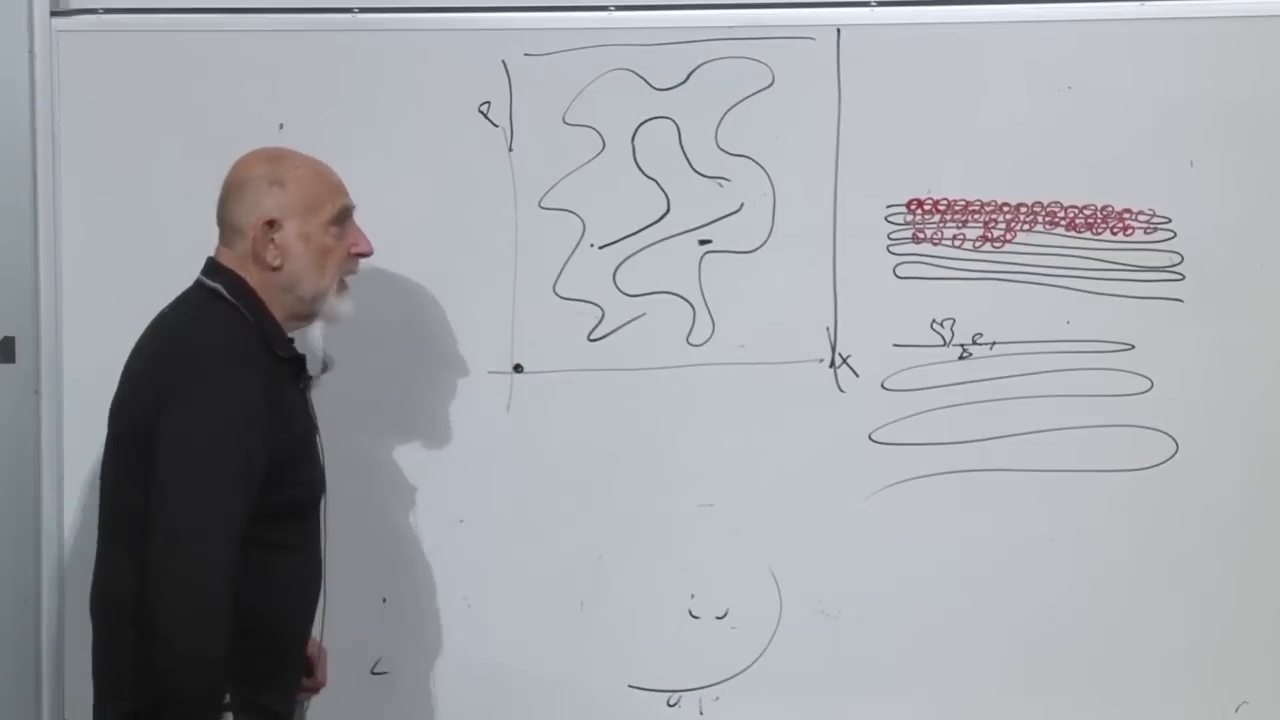
\includegraphics[width=0.90\textwidth]{lecture_07_figure_14.png}
\caption{コンパクトな特別な状態が、有界な到達可能領域を通して複雑なフィラメントへと発展する一方、粗視化されたセルははるかに大きな面積に広がる。}
\lectureframe{01:33:10}
\end{figure}

二つの留保が重要である。カオスそれ自体は、すべての軌道がすべての到達可能な近傍を訪れることを証明しない。そのより強いサンプリングの主張には、エルゴード性または混合性が必要である。また、すべての物理系がカオス的であるわけでもない。一般的な多体系気体と理想化されたビリヤードが意図された設定を与え、そこでは混合性が有用な物理的期待である。

\section{再帰は不可逆性を廃しない}

すべての空気分子が、特別に用意された速度パターンをもって一つの隅から始まるとしよう。衝突はすぐにそれらを部屋中に広げ、粗視化された記述は平衡に達する。有限の測度保存相空間では、ポアンカレの再帰定理は、ほとんどすべての初期点がその出発点にいくらでも近く戻ると述べる。許容誤差\(\epsilon>0\)に対して、再帰時間\(t_R(\epsilon)\)は定理の仮定のもとで有限であるが、巨視的な系では途方もなく大きい。無限に精密な点への厳密な回帰は、必要でもなく、一般に期待もされない。

\begin{classroomqa}
\audiencequestion{ビリヤードの例では、手球を突くことはエネルギーを注入し、閉じた発展を損なうのではないか。}
\lecturerresponse{選ばれた初期状態は、そのエネルギーがすでに含まれた状態で、突いた直後から始まる。再帰はその後の孤立した理想化されたビリヤード力学に関わり、初期状態の近くへの回帰は、選ばれた許容誤差の範囲内で手球がラックに近づくことに相当する配置を含む。
\lecturetimestamp{01:35:37--01:35:55}}
\end{classroomqa}

\begin{classroomqa}
\audiencequestion{気体がやがて隅に戻りうるならば、われわれは情報を失ったのか、そして系は本当に可逆なのか。}
\lecturerresponse{微視的力学は全体を通じて可逆のままである。粗視化エントロピーは、われわれが細かな相関を分解するのをやめるために上昇しうるが、きわめて稀な揺らぎは系をその特別な初期マクロ状態の近くへ戻しうる。したがって、再帰と粗視化された不可逆性は両立する。
\lecturetimestamp{01:37:34--01:38:15}}
\end{classroomqa}

これがボルツマンの本質的な定式化へと導く。エントロピーは論理的に可能なあらゆる瞬間に増大するわけではない。大きな系の非平衡マクロ状態が与えられると、圧倒的に多くの両立する微視的継続は、より特別なものへ向かうよりも、より大きなマクロ状態へ向かう。エントロピーは\emph{おそらく}増大する。下方への揺らぎと再帰は許されるが、その確率と時間スケールは、通常の巨視的経験においてそれらを見えなくする。可逆性の問題は統計力学の偉大な歴史的苦闘の一つであり、ボルツマンに重くのしかかった。その歴史的つながりは、彼の生涯についての単純な因果的主張に変えられるべきではない。

\section{カオスが意味するもの}

より操作的なカオスの定義としては、二つの初期位相点が\(\delta\Gamma(0)\)だけ異なるとき、カオス的な方向は典型的には、線形化された分離が意味を持つ領域で
\begin{equation}
 \lVert\delta\Gamma(t)\rVert
 \sim e^{\lambda t}\lVert\delta\Gamma(0)\rVert,
 \qquad \lambda>0,
 \label{eq:sm7-lyapunov-growth}
\end{equation}
となる。数\(\lambda\)はリアプノフ指数である。時間\(t\)を予測するには、初期データに必要な精度はおよそ\(e^{-\lambda t}\)でスケールする。力学法則の精度も重要である。モデルの誤差は初期条件の誤差とともに増幅される。天気はよく知られた例である。

\begin{classroomqa}
\audiencequestion{\emph{ほとんどの}系がカオス的であると言う原理は存在するのか、それともそれは単に経験的なものなのか。}
\lecturerresponse{カオス的および非カオス的なハミルトニアンは無限に存在し、そもそも\emph{ほとんど}という語にはハミルトニアンの空間上の測度が必要である。複雑な相互作用系はしばしばカオス的であるが、すべてのハミルトニアンを目視で分類するような初等的で普遍的な判定法は存在しない。
\lecturetimestamp{01:39:27--01:40:49}}
\end{classroomqa}

\begin{classroomqa}
\audiencequestion{この議論において\emph{カオス的}とは正確には何を意味するのか。}
\lecturerresponse{近接する位相軌道は、長時間予測には初期条件の知識を指数関数的に改善することを要するほど急速に分離する。調和振動子は対照的である。隣接する位相点はともに回転し、近くにとどまる。厳密な二体ケプラー問題も非カオス的であるが、一般の三体問題にはカオス的な領域がある。
\lecturetimestamp{01:40:50--01:43:45}}
\end{classroomqa}

\begin{classroomqa}
\audiencequestion{運動法則も初期条件と同様に高い精度で知られていなければならないのか。}
\lecturerresponse{はい。両方の誤差源が力学を通じて伝播し、カオス的発展は両方を増幅する。
\lecturetimestamp{01:43:46--01:43:55}}
\end{classroomqa}

二重振り子は鮮やかな例を与える。通常の振り子は可積分で予測可能である。二つ目の振り子を加えると、ほとんど同時に始まった軌道が最終的には異なる仕方でエネルギーを移動し、まったく異なる方向へ向かうことがある。

\begin{figure}[t]
\centering
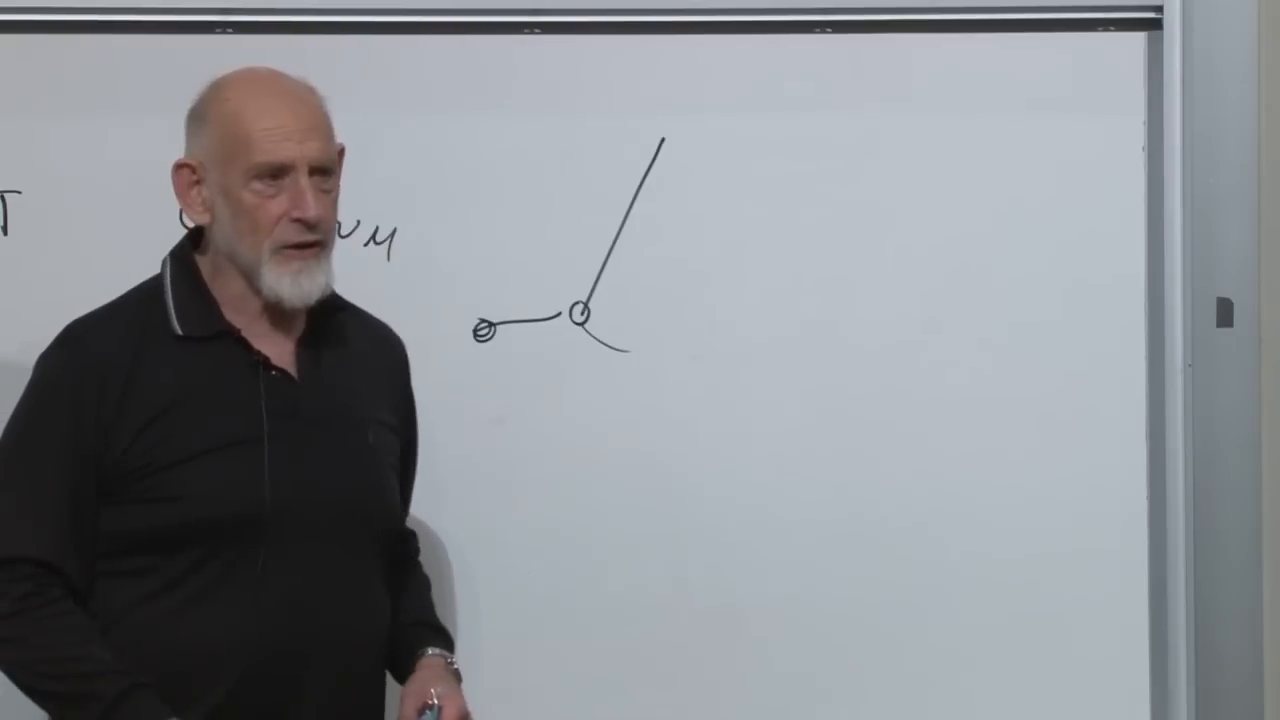
\includegraphics[width=0.90\textwidth]{lecture_07_figure_15.png}
\caption{決定論的カオスの具体例としての二重振り子。}
\lectureframe{01:44:40}
\end{figure}

\begin{classroomqa}
\audiencequestion{なぜある力学系はカオス的であり、別の系はそうでないのか。}
\lecturerresponse{それはハミルトニアンとその不変構造の性質であり、摩擦や実験ノイズの結果ではない。それを決定することは数学的に困難でありうる。複雑さは示唆的であるが証明ではない。
\lecturetimestamp{01:44:03--01:45:58}}
\end{classroomqa}

\begin{classroomqa}
\audiencequestion{摩擦のない理想的な二重振り子も依然としてカオス的か。}
\lecturerresponse{はい。散逸は必要でない。厳密な決定論的ハミルトニアン運動は初期条件への敏感な依存性を持ちうる。無限精度の初期データがあれば軌道は無限に決定されるが、有限精度では予測の地平は有限である。
\lecturetimestamp{01:45:57--01:47:54}}
\end{classroomqa}

\begin{classroomqa}
\audiencequestion{カオスは閉形式解を持たないことと同じか。}
\lecturerresponse{いいえ。カオス系は一般に大域的に有用な閉形式の軌道を持たないが、解析的可解性と敏感な依存性は異なる性質である。カオスは単に公式を書けないことによってではなく、軌道の分離によって力学的に診断される。
\lecturetimestamp{01:48:20--01:49:23}}
\end{classroomqa}

\begin{classroomqa}
\audiencequestion{遍在するカオスは、丘の不安定な頂上で正確に釣り合うこととどう異なるのか。}
\lecturerresponse{丘の頂上は一つの例外的な不安定状態である。そこから離れれば、近接する軌道が急速に分離する必要はない。カオス的領域では、不安定性は軌道に沿って典型的であり、近接する位相点は繰り返し分離する。正のリアプノフ指数がその持続的な成長を捉えている。
\lecturetimestamp{01:49:27--01:50:11}}
\end{classroomqa}

\section{微視的運動から統計法則へ}

音速の見積もりは、微視的な熱運動が巨視的な伝播スケールをどのように定めるかを示し、またその問いは指定されなければならない熱力学的導関数を明らかにした。次に振動子は、古典的等分配の到達範囲と失敗を示した。量子準位間隔は硬いモードを凍結させ、熱容量が温度とともに変化する理由を説明し、無限に多くの高周波モードが無限の熱エネルギーを運ぶことを防ぐ。

厳密な微視的物理から有効な巨視的記述への同じ進行が、第二法則の核心にある見かけの矛盾を解決する。ハミルトン流は厳密な位相空間体積を保存し、可逆のままである。カオス的伸長は巨視的記述が保持するよりも細かい相関を生み出すため、粗視化された占有領域は成長する。再帰は稀な回帰が禁じられていないことを保証する。確率は、なぜそれらが通常の経験を定義しないのかを説明する。第二法則は新しい不可逆的な微視的力ではない。それは、膨大な数の自由度を持つ系における特別な巨視的初期条件に対する、圧倒的に信頼できる統計的な進化の方向である。